\section{Design: Research Methodology Sketch}
\label{sec:methods}
The steps below outline the research methodology that will be adopted for the implementation of the proposed model. \hyperref[fig:image_label]{Figure 1} illustrates the architecture of the project work flow.

\subsection{Research Design and Intent }
The main research questions have been stated in \hyperref[subsec: research qs]{section 3.6}. The research design has been formulated by conducting a critical analysis of previous studies and identifying potential research gaps. It was evident that future research could focus on explainable AI and risk stratification on machine learning models. A two-way approach will be adopted for model development. The initial focus will be on traditional machine learning models, followed by integrating deep learning techniques for analysing tabular data in healthcare.

Traditional Machine Learning Models such as Decision trees, random forests and other popular \gls{ml} techniques will be used. 
\begin{itemize}
    \item \textbf{Random Forest}: A Random Forest is a learning technique that creates multiple decision trees and combines their results. It is used to boost prediction accuracy and reduce overfitting. 
    \item \textbf{Decision Tree}: A Decision Tree is used to classify \gls{cvd} risk by using a tree-like structure where each node is based on certain patient criteria.
\end{itemize}
\\

Deep Learning Model
\begin{itemize}
    \item \textbf{Fully Connected Neural Network}: It is a type of neural network where every neuron in the current layer is connected to every neuron in the previous and next layer. It enhances prediction accuracy by capturing non-linear relationships in the data. \citep{geeksforgeeks_fully_connected_layer}
\end{itemize}

\subsection{Research Methodology}
\subsubsection{Data Acquisition and Preprocessing}
The primary datasets considered include the Heart Disease dataset which was obtained from \gls{uci} Machine Learning Repository \citep{janosi1989heart}, Framingham dataset \cite{kaggle2023framingham} and Statlog heart disease dataset \citep{uci2023statlog}. The \gls{uci} Heart Disease dataset, ethically cleared and sourced from reputable sources, includes 14 attributes and 303 rows, including patient heart disease factors like age, cholesterol, blood pressure, and diabetes, to enhance the model's risk assessment. This stage involves cleaning the dataset to address null values and inconsistencies within the data. Identifying missing and duplicate values is essential to prevent bias during model training. The dataset will be divided into training and testing subsets which will be used to train and test the model's performance respectively.

\subsubsection{Feature Selection} In this stage, significant features are identified and selected. This step is crucial as it enhances the model’s accuracy. The core features are presented using explainable AI techniques in the form of graphs to facilitate better understanding. This increases transparency and user confidence in the model by helping users understand which features are highly influencing its predictions.

\subsubsection{Model Development} Next, the model will be developed using a wide range of machine learning techniques, including Random Forests and Decision Trees. A fully connected neural network will be implemented using deep learning techniques. This phase will use \gls{xai} techniques to examine how different algorithms handle attributes and prediction processes, ensuring that the model's outputs remain comprehensible even as complexity grows. SHapley Additive exPlanations (SHAP) is a powerful explainable \gls{ai} technique that offers clarity to the opaque predictions of \gls{ml} models \citep{yasunobu2022shapley}. Patients will be classified using risk categories such as low, medium, and high enabling the model to stratify patients by their risk of developing cardiovascular disease. 

\subsubsection{Model Testing and Evaluation} The model will be tested by using a subset of the dataset that was reserved earlier for testing purposes. The predictive performance of the developed model will be assessed through standard quantitative evaluation metrics, such as accuracy, precision, and recall. \hyperref[sec:eval]{Chapter 5} details on further analysis of the evaluation strategy used. 

\subsection{Development Tools} Python will be used as the primary programming language for this project, due to the extensive range of libraries it offers for machine learning and data analysis, including tools like scikit-learn, tensorflow/keras, pandas, and numpy.  Github will be used as a code repository.

\subsection{Significance: Aiming for Clinical Utility}
The study aims to develop a practical model for early heart disease risk prediction, integrating \gls{shap} values and risk stratification. Hence, it enables clinicians to assess patient risk more accurately and deliver personalized treatment plans in cardiovascular care,  bridging the gap between predictive
performance and interpretability.
\begin{figure}[h!]
    \centering
    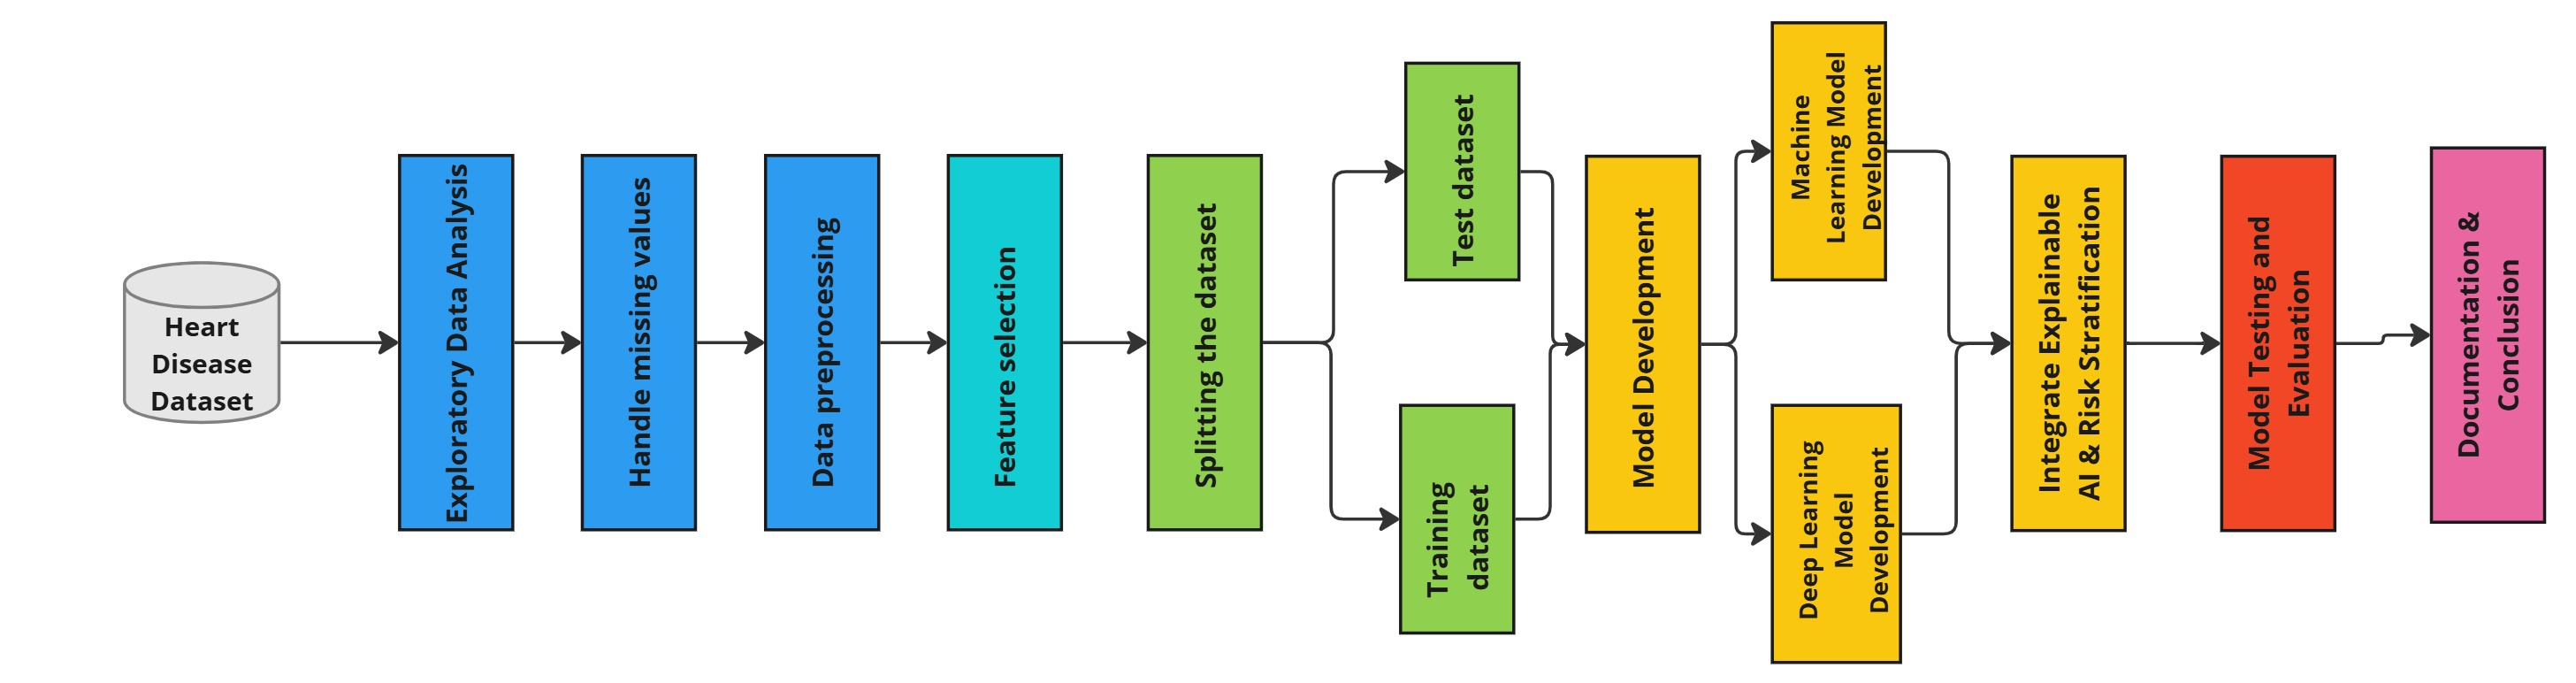
\includegraphics[width=0.8\textwidth]{text/main_body/images/Flowchart.jpg} 
    \caption{Model Development Architecture}
    \label{fig:image_label}
\end{figure}
